\documentclass[a4paper]{article}

%% Language and font encodings
\usepackage[english]{babel}
\usepackage{amsthm, amsfonts, xpatch}
\usepackage[utf8x]{inputenc}
\usepackage[T1]{fontenc}
\usepackage{listings}
\usepackage{algpseudocode, algorithm}
\usepackage{mathtools}
\usepackage{enumerate}
\usepackage{tabu}
\usepackage{xcolor}
\usepackage{tikz, tikz-qtree}
\usetikzlibrary{arrows, automata, positioning}
\usepackage{graphviz}
\usepackage{subfig}
\usepackage{blindtext}
%% Sets page size and margins
\usepackage[a4paper,top=3cm,bottom=2cm,left=3cm,right=3cm,marginparwidth=1.75cm]{geometry}
\usepackage{multicol}

%% Useful packages
\usepackage{amsmath}
\usepackage{graphicx}
\usepackage[colorinlistoftodos]{todonotes}
\usepackage[colorlinks=true, allcolors=blue]{hyperref}

\newenvironment{solution}{\begin{proof}[\textnormal{\textbf{Solution}}]}{\end{proof}}
\newenvironment{exercise}[1]{\begin{proof}[\textnormal{\textbf{Exercise #1:}}]\phantom{\qedhere}}{\end{proof}}

\renewcommand\thesubfigure{\arabic{subfigure}}
\theoremstyle{definition}
\newtheorem{definition}{Definition}[subsection]
\newtheorem{theorem}{Theorem}[subsection]
\newtheorem{lemma}{Lemma}

\begin{document}
\begin{titlepage}\pagenumbering{gobble}
	\centering
	{\scshape\LARGE University of Houston\par}
	\vspace{1cm}
	{\scshape\Large Notes \par}
	\vspace{1.5cm}
	{\huge\bfseries COSC 3340 \par}
	{\huge\bfseries Intro. to Automata and Computability \par}
	\vspace{0.5cm}
	{\large\bfseries Ernst Leiss\par}
	\vspace{1cm}
	{\Large\itshape Khalid Hourani}
	\vspace{0.5cm}
	{\large \par} %date
	\vfill
% Bottom of the page
\end{titlepage}

\tableofcontents
\newpage\pagenumbering{arabic}

\section{Formal Languages}\label{sec:introduction}
\subsection{Introduction}\label{subsubsec:introduction}
\begin{definition}
 An \textbf{Alphabet} is a finite, non-empty set of atomic symbols.
\end{definition}

\begin{definition}
 A \textbf{word} or \textbf{string} is any finite sequence of symbols from an alphabet. 
\end{definition}

\begin{definition}
 The \textbf{length} of a string, \(s\), denoted \(\abs{s}\), is the number of symbols in \(s\). 
\end{definition}

\begin{definition}
 Given strings \(s=s_1s_2\hdots s_n\) and \(t=t_1t_2\hdots t_m\), their \textbf{concatenation} is defined 
 
 \[s\cdot t=s_1s_2\cdots s_n t_1t_2\cdots t_m\]
\end{definition}

We denote by \(\varepsilon \) the \textbf{empty string}, the unique string of 0 characters. 

\begin{definition}
 Let \(A\) be any alphabet. The \textbf{Kleene Closure} of \(A\), denoted \(A^*\), is the set of all strings of any length over \(A\).  
\end{definition}

\begin{theorem}
 Let \(A\) be any finite set. Then \(A^*\) is countably infinite. 
\end{theorem}

\begin{proof}
 That \(A^*\) is infinite is straightforward: since \(A\) is non-empty, take \(a\in A\). Then \[ \{a, aa, aaa, \hdots \}\subseteq A^*\]
 
 To see that it is countable, we first write \(\abs{A}=n\). Now, consider the set of all strings of length 0. This is simply \( \{\varepsilon \} \). Moreover, there are \(n\) strings of length 1, \(n^2\) strings of length 2, \(n^3\) strings of length 3, and so on. Thus, we map \(\varepsilon \) to 0, the strings of length 1 to \(1, 2, \hdots, n\), the strings of length 2 to \(n+1, n+2, \hdots, n+n^2\), the strings of length 3 to \(n+n^2+1, n+n^2+2,\hdots, n+n^2+n^3\), and so on. This is a bijection from \(A^*\) to \(\mathbb{N}\), which completes the proof.
\end{proof}

\begin{definition}
 Given an alphabet \(A\), a \textbf{formal language} or simply \textbf{language} \(L\) is any subset of \(A^*\). 
\end{definition}

\begin{theorem}
 Given an alphabet \(A\), the set of languages over \(A\) is uncountable. 
\end{theorem}

\begin{proof}
 Suppose, by way of contradiction, that the set of languages were countable, i.e., that we can enumerate the set as \( \{L_1, L_2, L_3, \hdots \} \). Consider the set of all strings \( \{s_1, s_2, s_3, \hdots \} \). Let \(L\) be the language defined as follows: 
 
\[s_i\in L\text{ if and only if } s_i\not\in L_i\]

 To see that \(L\) is not in the above list, consider \(s_i\). If \(s_i\) is in \(L\), then \(s_i\) is not in \(L_i\), by construction, and \(L\neq L_i\). Similarly, if \(s_i\) is not in \(L\), then \(s_i\) must be in \(L_i\), by construction, and \(L\neq L_i\). In other words, for all \(i\), \(L\neq L_i\). Then \(L\) is not in the above list, which is a contradiction. Hence, the set of languages is uncountable. 
\end{proof}

All set operations, such as union, intersection, complement, set-difference, etc.\@ can be applied to languages, since languages are simply subsets of a Kleene Closure of an alphabet.

\begin{definition}
 Given two languages \(L_1\) and \(L_2\), the concatenation \(L_1\cdot L_2\) is given by
 
 \[L_1\cdot L_2=\{s\cdot t \mid s\in L_1\text{ and } t\in L_2\} \]
\end{definition}

Clearly, we have 

\begin{align*}
    L\cdot\emptyset &= \emptyset = \emptyset\cdot L\\
    L\cdot \{\varepsilon \} &= L = \{\varepsilon \}\cdot L
\end{align*}

Note that \(L_1\cdot L_2\) is not the same as \(L_1\times L_2\). Let \(L_1=L_2=\{\varepsilon, 0, 00\} \). Then

\[L_1\times L_2=\{(\varepsilon, \varepsilon), (\varepsilon, 0), (\varepsilon, 00), (0, \varepsilon), (0, 0), (0, 00), (00, \varepsilon), (00, 0), (00, 00)\} \]

whereas 

\[L_1\cdot L_2=\{\varepsilon, 0, 00, 000, 0000\} \]

\begin{definition}
 Given a language \(L\), the \textbf{Kleene Closure} of \(L\), \(L^*\), is 
 
 \[L^*=\bigcup_{i=0}^{\infty}L^i\]
 
 where \[L^i = \begin{cases} \{\varepsilon \} &\mbox{if } i = 0 \\
L \cdot L^{i-1} & \mbox{otherwise }\end{cases}\]
\end{definition}

Note that, while \(0^0\) is normally left undefined, we define \(\emptyset^0=\{\varepsilon \} \).

\begin{theorem}
 \(L^*\) is finite if and only if \(L=\emptyset \) or \(L=\{\varepsilon \} \).
\end{theorem}

\begin{proof}
 If \(L=\emptyset \), then \(L^i=\emptyset^i=\emptyset \) for \(i>0\). Then 
 
 \begin{align*}\emptyset^*&=\bigcup_{i=0}^{\infty}\emptyset^i\\
                          &=\emptyset^0\cup\bigcup_{i=1}^{\infty}\emptyset^i\\
                          &=\{\varepsilon \}\cup\bigcup_{i=1}^{\infty}\emptyset \\
                          &=\{\varepsilon \}
\end{align*}

Similarly, if \(L=\{\varepsilon \} \), then \(L^i=\{\varepsilon \} \) for all \(i\), and 

 \begin{align*}{\{\varepsilon \}}^*&=\bigcup_{i=0}^{\infty}{\{\varepsilon \}}^i\\
                          &=\bigcup_{i=1}^{\infty}\{\varepsilon \} \\
                          &=\{\varepsilon \}
\end{align*}

However, if \(L\) is neither \(\emptyset \) nor \( \{\varepsilon \} \), then there exists a string \(s\in L\) with length at least 1. Then \(s, ss, sss, \hdots \), are in \(L^*\), hence \(L^*\) is infinite.
\end{proof}

\subsection{Regular Languages}\label{subsec:regular-languages}
\subsubsection{Finite Automata}\label{subsubsec:finite-automata}

\begin{definition}
A \textbf{Deterministic Finite-State Automata} (DFA) or \textbf{Finite-State Machine} is a quintuple $(A, Q, \tau, q_0, \mathcal{F})$ where 

\begin{align*}
    &A\text{ is the }\textbf{alphabet}\\
    &Q\text{ is a finite, non-empty }\textbf{set of states}\\
    &\tau:Q\times A\to Q\text{ is the }\textbf{transition function }\\
    &q_0\text{ is the }\textbf{initial state}\\
    &\mathcal{F}\subseteq Q\text{ is the set of }\textbf{final states}
\end{align*}
\end{definition}
We can extend $\tau$ as follows: 

$\tau^*:Q\times A^*\to Q$

\[\tau^*(q, s) = \begin{cases} q &\mbox{ if } s=\varepsilon\\
                             \tau^*(\tau(q, s_0), s') &\mbox{ if } s=s_0\cdot s'\end{cases}\]

We proceed informally and use $\tau$ to refer to $\tau^*$. 

Consider the following DFA:

\begin{center}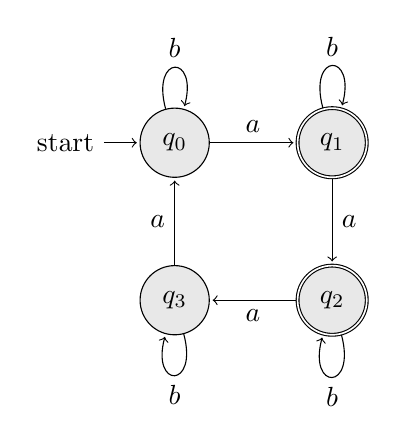
\begin{tikzpicture}[shorten >=1pt,node distance=2cm,on grid,auto]
  \tikzstyle{every state}=[fill={rgb:black,1;white,10}]

  \node[state,initial](q_0){$q_0$};
  \node[state, accepting](q_1)[right of=q_0]{$q_1$};
  \node[state, accepting](q_2)[below of=q_1]{$q_2$};
  \node[state](q_3)[left of=q_2]{$q_3$};

  \path[->]
  (q_0) edge                node {$a$}  (q_1)
        edge  [loop above]  node {$b$}  ()
  (q_1) edge                node {$a$}  (q_2)
        edge  [loop above]  node {$b$}  ()
  (q_2) edge                node {$a$}  (q_3)
        edge  [loop below]  node {$b$}  ()
  (q_3) edge                node {$a$}  (q_0)
        edge  [loop below]  node {$b$}  ();
\end{tikzpicture}\end{center}

The figure indicates that we begin at state $q_0$. The double-circles for states $q_1$ and $q_2$ indicate that they are accepting or final states. An arrow indicates the state to move to after receiving an input. For example, if we receive the input string $abba$, we begin at state $q_0$ and receive $a$, so we move to state $q_1$. We then receive $b$ and stay in $q_1$. We repeat this for the next symbol, $b$, and then move to $q_2$ upon receiving the final $a$. Since $q_2$ is a final state, we say that this DFA \textbf{accepts} the string $abba$. 

We can represent the above DFA using a table, as follows:

\begin{center}\begin{tabular}{r|c c r}
         & $a$ & $b$ & \\\hline
    $\to q_0$ & $q_1$ & $q_0$ & 0 \\
    $q_1$ & $q_2$ & $q_1$ & 1 \\
    $q_2$ & $q_3$ & $q_2$ & 1\\
    $q_3$ & $q_0$ & $q_3$ & 0\\
\end{tabular}\end{center}

The first column indicates the states, while the first row indicates the symbols. The final column indicates whether a state is accepting: 0 refers to a non-final state, 1 to a final state. The remaining values indicate the transition function $\tau$, e.g. $\tau(q_0, a)=q_1$, indicated by the entry corresponding to row $q_0$ and column $a$. Finally, the arrow pointing to $q_0$ indicates that it is the starting position. 

\begin{definition}
Let $\underset{\sim}{D}$ be some DFA. Then $L(\underset{\sim}{D})$, the language accepted by the DFA, is \[\{s\in A^*|\tau(q_0, s)\in \mathcal{F}\}\]
\end{definition}

\begin{definition}
A language is \textbf{regular} if and only if there exists a DFA that accepts it.
\end{definition}

\begin{definition}
A \textbf{Non-Deterministic Finite-State Automata} (NFA) is a quintuple $(A, Q, \tau, q_0, \mathcal{F})$ where 
\end{definition}

\begin{align*}
    &A\text{ is the }\textbf{alphabet}\\
    &Q\text{ is a finite, non-empty }\textbf{set of states}\\
    &\tau:Q\times A\to 2^Q\text{ is the }\textbf{transition function }\\
    &q_0\text{ is the }\textbf{initial state}\\
    &\mathcal{F}\subseteq Q\text{ is the set of }\textbf{final states}
\end{align*}

We can extend $\tau$ as follows: 

$\tau^*:2^Q\times A^*\to 2^Q$

\[\tau^*(P, s) = \begin{cases} P &\mbox{ if } s=\varepsilon\\
                             \tau^*\left(\displaystyle\bigcup_{q\in P}\tau(q, s_0), s'\right) &\mbox{ if } s=s_0\cdot s'\end{cases}\]

We proceed informally and use $\tau$ to refer to $\tau^*$. 

Consider the following NFA:

\begin{center}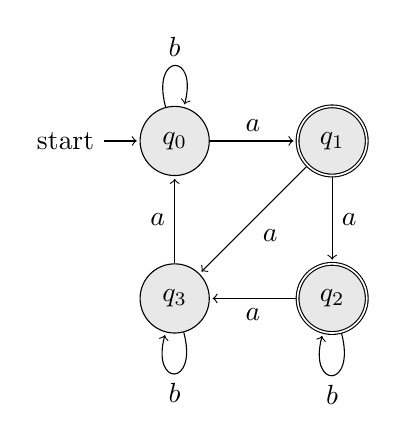
\begin{tikzpicture}[shorten >=1pt,node distance=2cm,on grid,auto]
  \tikzstyle{every state}=[fill={rgb:black,1;white,10}]

  \node[state, initial](q_0){$q_0$};
  \node[state, accepting](q_1)[right of=q_0]{$q_1$};
  \node[state, accepting](q_2)[below of=q_1]{$q_2$};
  \node[state](q_3)[left of=q_2]{$q_3$};

  \path[->]
  (q_0) edge                node {$a$}  (q_1)
        edge  [loop above]  node {$b$}  ()
  (q_1) edge                node {$a$}  (q_2)
        edge                node {$a$}  (q_3)
  (q_2) edge                node {$a$}  (q_3)
        edge  [loop below]  node {$b$}  ()
  (q_3) edge                node {$a$}  (q_0)
        edge  [loop below]  node {$b$}  ();
\end{tikzpicture}\end{center}

The diagrams for an NFA and DFA follow the same notation. However, the notation for the table differs slightly:

\begin{center}\begin{tabular}{r|c c r}
         & $a$ & $b$ & \\\hline
    $\to q_0$ & $q_1$ & $q_0$ & 0 \\
    $q_1$ & $q_2q_3$ & $\emptyset$ & 1 \\
    $q_2$ & $q_3$ & $q_2$ & 1\\
    $q_3$ & $q_0$ & $q_3$ & 0\\
\end{tabular}\end{center}

The values of the transition function are now sets. We informally refer to the set $\{q_0\}$ by $q_0$, and similarly the set $\{q_2, q_3\}$ by $q_2q_3$. In some cases, to avoid ambiguity, we will use commas, e.g. we may represent $\{q_2, q_3\}$ as $q_2,q_3$. We similarly say, given a string $s$, if there exists a path through an NFA that ends in a final state, we say that the NFA \textbf{accepts} $s$.

Similarly, we define the set of languages accepted by an NFA $\underset{\sim}{N}$, $L(\underset{\sim}{N})$, as \[L(\underset{\sim}{N}) = \{s\in A^*|\tau(q_0, s)\cap\mathcal{F}\neq\emptyset\}\]

It should be clear that each DFA is an NFA, but the reverse is not true. However, we can convert an NFA to a DFA on the powerset $2^{\mathcal{Q}}$ by using the \textbf{subset construction}: begin with the initial state and traverse the NFA, adding unseen states to the left-most column until all paths have been exhausted. For example, with our NFA above, we begin with:

\begin{center}\begin{tabular}{r|c c r}
         & $a$ & $b$ & \\\hline
    $\to q_0$ & $q_1$ & $q_0$ & 0 \\
\end{tabular}\end{center}

$q_0$ has already been seen, so we ignore it. $q_1$ is new, so we add it to the table:

\begin{center}\begin{tabular}{r|c c r}
         & $a$ & $b$ & \\\hline
    $\to q_0$ & $q_1$ & $q_0$ &  \\
          $q_1$ &       &       & 
\end{tabular}\end{center}

We now visit the corresponding states of $q_1$, which are $q_2q_3$ and $\emptyset$, both of which have not yet been visited. 

\begin{center}\begin{tabular}{r|c c r}
         & $a$ & $b$ & \\\hline
    $\to q_0$ & $q_1$ & $q_0$ &  \\
          $q_1$ & $q_2q_3$ & $\emptyset$ & \\
          $q_2q_3$ & & & \\
          $\emptyset$ & & &
\end{tabular}\end{center}

When $q_2$ receives $a$, it transitions to state $q_3$. When $q_3$ receives $a$, it transitions to state $q_0$, so $q_2q_3$ transitions to $q_0q_3$. Similarly, $q_2q_3$ transitions to state $q_2q_3$ when it receives $b$.

\begin{center}\begin{tabular}{r|c c r}
         & $a$ & $b$ & \\\hline
    $\to q_0$ & $q_1$ & $q_0$ &  \\
          $q_1$ & $q_2q_3$ & $\emptyset$ & \\
          $q_2q_3$ & $q_0q_3$ & $q_2q_3$ & \\
          $\emptyset$ & & &
\end{tabular}\end{center}

The empty set transitions to the empty set, by definition. 

\begin{center}\begin{tabular}{r|c c r}
         & $a$ & $b$ & \\\hline
    $\to q_0$ & $q_1$ & $q_0$ &  \\
          $q_1$ & $q_2q_3$ & $\emptyset$ & \\
          $q_2q_3$ & $q_0q_3$ & $q_2q_3$ & \\
          $\emptyset$ & $\emptyset$ & $\emptyset$ &
\end{tabular}\end{center}

$q_0q_3$ has not yet been visited, so we add it to the left-most column:

\begin{center}\begin{tabular}{r|c c r}
         & $a$ & $b$ & \\\hline
    $\to q_0$ & $q_1$ & $q_0$ &  \\
          $q_1$ & $q_2q_3$ & $\emptyset$ & \\
          $q_2q_3$ & $q_0q_3$ & $q_2q_3$ & \\
          $\emptyset$ & $\emptyset$ & $\emptyset$ &\\
          $q_0q_3$ & & & 
\end{tabular}\end{center}

Then we visit its corresponding states:

\begin{center}\begin{tabular}{r|c c r}
         & $a$ & $b$ & \\\hline
    $\to q_0$ & $q_1$ & $q_0$ &  \\
          $q_1$ & $q_2q_3$ & $\emptyset$ & \\
          $q_2q_3$ & $q_0q_3$ & $q_2q_3$ & \\
          $\emptyset$ & $\emptyset$ & $\emptyset$ &\\
          $q_0q_3$ & $q_0q_1$ & $q_0q_3$ & 
\end{tabular}\end{center}

Continuing, we end with the following DFA:

\begin{center}\begin{tabular}{r|c c r}
         & $a$ & $b$ & \\\hline
    $\to q_0$ & $q_1$ & $q_0$ &  \\
          $q_1$ & $q_2q_3$ & $\emptyset$ & \\
          $q_2q_3$ & $q_0q_3$ & $q_2q_3$ & \\
          $\emptyset$ & $\emptyset$ & $\emptyset$ &\\
          $q_0q_3$ & $q_0q_1$ & $q_0q_3$ & \\
          $q_0q_1$ & $q_1q_2q_3$ & $q_0$ & \\
          $q_1q_2q_3$ & $q_0q_2q_3$ & $q_2q_3$ & \\
          $q_0q_2q_3$ & $q_0q_1q_3$ & $q_0q_2q_3$ & \\
          $q_0q_1q_3$ & $q_0q_1q_2q_3$ & $q_0q_3$ & \\
          $q_0q_1q_2q_3$ & $q_0q_1q_2q_3$ & $q_0q_2q_3$ & \\
\end{tabular}\end{center}

However, we need to include the accepting states. The accepting states of the NFA are $q_1$ and $q_2$, and thus any state including either state is accepting:

\begin{center}\begin{tabular}{r|c c r}
         & $a$ & $b$ & \\\hline
    $\to q_0$ & $q_1$ & $q_0$ & 0 \\
          $q_1$ & $q_2q_3$ & $\emptyset$ & 1 \\
          $q_2q_3$ & $q_0q_3$ & $q_2q_3$ & 1 \\
          $\emptyset$ & $\emptyset$ & $\emptyset$ & 0\\
          $q_0q_3$ & $q_0q_1$ & $q_0q_3$ & 0 \\
          $q_0q_1$ & $q_1q_2q_3$ & $q_0$ & 1 \\
          $q_1q_2q_3$ & $q_0q_2q_3$ & $q_2q_3$ & 1 \\
          $q_0q_2q_3$ & $q_0q_1q_3$ & $q_0q_2q_3$ & 1 \\
          $q_0q_1q_3$ & $q_0q_1q_2q_3$ & $q_0q_3$ & 1 \\
          $q_0q_1q_2q_3$ & $q_0q_1q_2q_3$ & $q_0q_2q_3$ & 1\\
\end{tabular}\end{center}

Note that an NFA does not necessarily admit a DFA with as many states. Consider the following example:

\begin{center}\begin{tabular}{r| c c r}
     & $a$ & $b$ & \\\hline
$\to 0$&$\{1,2,\hdots,n\}$ & 0 & 0 \\
     1 & 2 & 1 & 0 \\
     2 & 3 & 2 & 0 \\
     \vdots & \vdots & \vdots & \vdots \\
     $i$ & $i + 1$ & $i$ & 0 \\
     \vdots & \vdots & \vdots & \vdots \\
     $n-1$ & $n$ & $n-1$ & 0 \\
     $n$ & 1 & $n$ & 1
\end{tabular}\end{center}

The NFA above admits the following DFA:

\begin{center}\begin{tabular}{r| c c r}
     & $a$ & $b$ & \\\hline
$\to 0$&$\{1,2,\hdots,n\}$ & 0 & 0 \\
     $\{1, 2,\hdots, n\}$ & $\{1, 2,\hdots, n\}$ & $\{1, 2,\hdots, n\}$ & 1 \\
\end{tabular}\end{center}

The above DFA contains only 2 states, despite the NFA containing $n+1$ states.

That every NFA admits a DFA which accepts the same language shows that the class of languages denoted by DFAs, $\mathcal{L}_{\text{DFA}}$, is the same as the class of languages denoted by NFAs, $\mathcal{L}_{\text{NFA}}$, i.e, that

\[\mathcal{L}_{\text{DFA}} = \mathcal{L}_{\text{NFA}}\]

For an NFA, there is no guarantee of a unique smallest NFA which accepts the same strings. However, for a DFA, such a notion exists.

Consider two states, $p$ and $q$, and corresponding $L_p$ and $L_q$, where $L_p$ has initial state $p$ and $L_q$ has initial state $q$. We say that $p$ and $q$ are distinguishable if there exists a string $s$ such that $s$ is in $L_p$ and not in $L_q$, or vice-versa. We use this notion to \textbf{reduce} a DFA.

Begin with a partition of $Q$ into subsets $\mathcal{F}$ and $Q-\mathcal{F}$, i.e., the accepting and rejecting states. For a pair of states $p, q$ if the result of transitioning $p$ and $q$ falls into different partitions, we partition the subset and continue.

For example, given the following DFA:

\begin{center}\begin{tabular}{r| c c r}
         & $a$ & $b$ & \\\hline
         $\to 0$ & 1 & 2 & 0\\
               1 & 2 & 3 & 1\\
               2 & 3 & 4 & 0\\
               3 & 0 & 5 & 1\\
               4 & 5 & 6 & 0\\
               5 & 6 & 7 & 1\\
               6 & 7 & 0 & 0\\
               7 & 4 & 1 & 1
    \end{tabular}\end{center}

We have two partitions:

\begin{center}\begin{tabular}{c|c|c|c|c|c|c|c}
\multicolumn{4}{c|}{Rejecting} & \multicolumn{4}{|c}{Accepting}\\\hline
\multicolumn{4}{c|}{0, 2, 4, 6} & \multicolumn{4}{|c}{1, 3, 5, 7}
\end{tabular}\end{center}

Now, 0 gets sent to the accepting partition by $a$ and to the rejecting partition by $b$. Similarly, 2, 4, and 6 get sent to the accepting partition by $a$ and to the rejecting partition by $b$. Thus, they belong to the same partition.

In the same vein, 1 gets sent to the rejecting partition by $a$ and to the accepting partition by $b$. Similarly, 3, 5, and 7 get sent to the rejecting partition by $a$ and to the accepting partition by $b$. Thus, our next partition is

\begin{center}\begin{tabular}{|c|c|c|c|c|c|c|c|}
\multicolumn{4}{|c|}{Rejecting} & \multicolumn{4}{|c|}{Accepting}\\\hline
\multicolumn{4}{|c|}{0, 2, 4, 6} & \multicolumn{4}{|c|}{1, 3, 5, 7}\\
\multicolumn{4}{|c|}{0, 2, 4, 6} & \multicolumn{4}{|c|}{1, 3, 5, 7}
\end{tabular}\end{center}

That our row is the same as the preceding one indicates that we have finished, and now have a minimal DFA. Call the first subset $p$ and the second $q$. When an element in $p$ receives $a$, it is sent to $q$. When it receives $b$, it is sent to $p$. Similar logic for $q$ gives our new DFA:

\begin{center}\begin{tabular}{r| c c r}
         & $a$ & $b$ & \\\hline
         $\to p$ & $q$ & $p$ & 0\\
               $q$ & $p$ & $q$ & 1\\
    \end{tabular}\end{center}

Recall that $p$ began as a subset of the rejecting elements and $q$ the accepting elements, which informs the last column of the above table.
    
Not all DFAs can be reduced. An obvious example is the above reduced DFA. For a less trivial example, consider the following DFA:
   
    \begin{center}\begin{tabular}{r| c c r}
         & $a$ & $b$ & \\\hline
         $\to 0$ & 1 & 2 & 0\\
               1 & 2 & 3 & 1\\
               2 & 3 & 4 & 0\\
               3 & 0 & 5 & 1\\
               4 & 5 & 6 & 0\\
               5 & 6 & 7 & 1\\
               6 & 7 & 0 & 0\\
               7 & 4 & 2 & 1
    \end{tabular}\end{center}

Begin, as in the previous problem, with two partitions:

\begin{center}\begin{tabular}{c|c|c|c|c|c|c|c}
\multicolumn{4}{c|}{Rejecting} & \multicolumn{4}{|c}{Accepting}\\\hline
\multicolumn{4}{c|}{0, 2, 4, 6} & \multicolumn{4}{|c}{1, 3, 5, 7}
\end{tabular}\end{center}

As in the previous problem, 0, 2, 4, and 6 get sent to the same partition under $a$ and $b$, respectively. Under $a$, 1, 3, 5, and 7 go to the rejecting partition. However, under $b$, 7 goes to the rejecting partition while 1, 3, and 5 go to the accepting partition, which means we must create a new partition for 7.  

\begin{center}\begin{tabular}{|c|c|c|c|c|c|c|c|}
\multicolumn{4}{|c|}{Rejecting} & \multicolumn{4}{|c|}{Accepting}\\\hline
\multicolumn{4}{|c|}{0, 2, 4, 6} & \multicolumn{4}{|c|}{1, 3, 5, 7}\\\hline
\multicolumn{4}{|c|}{0, 2, 4, 6} & \multicolumn{3}{|c|}{1, 3, 5} & 7
\end{tabular}\end{center}

We continue the process, noting that there is no need to consider singletones, i.e., the partition $\{7\}$ is already in its finale state. Under $a$, 0, 2, and 4 get sent to the $\{1, 3, 5\}$ partition. Under $b$, they get sent to the $\{0, 2, 4, 6\}$ partition. However, 6 gets sent to the $\{7\}$ partition, and so it must be partitioned separately. Similarly, 1 and 3 get sent to the $\{0, 2, 4, 6\}$ partition under $a$, and to the $\{1, 3, 5\}$ partition under b. 5, on the other hand, gets sent to the $\{7\}$ partition, and must be partitioned separately. In total, we have:

\begin{center}\begin{tabular}{|c|c|c|c|c|c|c|c|}
\multicolumn{4}{|c|}{Rejecting} & \multicolumn{4}{|c|}{Accepting}\\\hline
\multicolumn{4}{|c|}{0, 2, 4, 6} & \multicolumn{4}{|c|}{1, 3, 5, 7}\\\hline
\multicolumn{4}{|c|}{0, 2, 4, 6} & \multicolumn{3}{|c|}{1, 3, 5} & 7\\\hline
\multicolumn{3}{|c|}{0, 2, 4} & 6 & \multicolumn{2}{|c|}{1, 3} & 5 & 7
\end{tabular}\end{center}

We continue:

\begin{center}\begin{tabular}{|c|c|c|c|c|c|c|c|}
\multicolumn{4}{|c|}{Rejecting} & \multicolumn{4}{|c|}{Accepting}\\\hline
\multicolumn{4}{|c|}{0, 2, 4, 6} & \multicolumn{4}{|c|}{1, 3, 5, 7}\\\hline
\multicolumn{4}{|c|}{0, 2, 4, 6} & \multicolumn{3}{|c|}{1, 3, 5} & 7\\\hline
\multicolumn{3}{|c|}{0, 2, 4} & 6 & \multicolumn{2}{|c|}{1, 3} & 5 & 7\\\hline
\multicolumn{2}{|c|}{0, 2} & 4 & \multicolumn{1}{c|}{6} & \multicolumn{1}{|c|}{1} & 3 & 5 & 7\\\hline
0 & 2 & 4 & \multicolumn{1}{c|}{6} & \multicolumn{1}{|c|}{1} & 3 & 5 & 7
\end{tabular}\end{center}

Notice that the reduced DFA has 8 states, like the original! This means that the original DFA is already reduced, and cannot be reduced further.

\subsubsection{Regular Expressions}
\begin{definition}
Given an alphabet $A$, we define a \textbf{regular expression}
\begin{enumerate}[(a)]
    \item \begin{itemize}
        \item $a\in A$ is a regular expression denoting the language $\{a\}$
        \item $\varepsilon$ is a regular expression denoting $\{\varepsilon\}$
        \item $\emptyset$ is a regular expression denoting $\emptyset$
    \end{itemize}
    
    \item If $\alpha$ and $\beta$ are regular expressions denoting the languages $L(\alpha)$ and $L(\beta)$, respectively, then 
    \begin{itemize}
        \item $\alpha\cup\beta$ denotes $L(\alpha)\cup L(\beta)$
        \item $\alpha\cdot\beta$ denotes $L(\alpha)\cdot L(\beta)$
        \item $\alpha^*$ denotes $L(\alpha)^*$
    \end{itemize}
\end{enumerate}
\end{definition}

By convention, we define precedence of the operations $\cup$, $\cdot$, and $^*$ in that order. Thus, \[b\cdot a^*\cup c=(b\cdot(a^*))\cup c)\]

A regular expression $\alpha$ over an alphabet $A$ denotes the set of languages which accept $\alpha$. Thus, we would like to construct an NFA $\underset{\sim}{N}$ such that $L(\underset{\sim}{N})=L(\alpha)$.

The following NFA rejects all strings but $a$:

\begin{center}\begin{tabular}{r| c c r}
      & $a$ & $b\neq a$ & \\\hline
      $\to q_0$ & $q_1$ & $\emptyset$ & 0\\
            $q_1$ & $\emptyset$ & $\emptyset$ & 1\\
 \end{tabular}\end{center}

An NFA for only $\varepsilon$ would appear as:

\begin{center}\begin{tabular}{r| c r}
      & $c\in A$ & \\\hline
      $\to q_0$ & $\emptyset$ & 1\\
 \end{tabular}\end{center}

And finally, an NFA for only $\emptyset$ is:

\begin{center}\begin{tabular}{r| c r}
      & $c\in A$ & \\\hline
      $\to q_0$ & $\emptyset$ & 0\\
 \end{tabular}\end{center}

Now, suppose we have an NFA for $\alpha$ and $\beta$. We wish to determine NFAs for $\alpha\cup\beta$, $\alpha\cdot\beta$, and $\alpha^*$. 

We define \begin{align*}
      \underset{\sim}{N_\alpha} &= (A, Q_{\alpha}, \tau_{\alpha}, q_0, \mathcal{F}_{\alpha})\\
      \underset{\sim}{N_\beta}  &= (A, Q_{\beta}, \tau_{\beta}, q_0, \mathcal{F}_{\beta})
\end{align*}

such that \begin{align*}
      L(\underset{\sim}{N_\alpha}) &= L(\alpha)\\
      L(\underset{\sim}{N_\beta})  &= L(\beta)\\
      Q_\alpha\cap Q_\beta&=\{q_0\}
\end{align*}

and clarify that these automata are non-returning, i.e., that $q_0\not\in\tau(q_0, s)$ for any $s$ of length 1 or greater.

We construct the \textbf{Union} \[\underset{\sim}{N_{\alpha\cup\beta}}=(A, Q_{\alpha\cup\beta}, \tau_{\alpha\cup\beta}, q_0, \mathcal{F}_{\alpha\cup\beta})\] 

where $Q_{\alpha\cup\beta}=Q_{\alpha}\cup Q_{\beta}$, $\mathcal{F}_{\alpha\cup\beta}=\mathcal{F}_{\alpha}\cup F_{\beta}$ and, for all $q\in Q_{\alpha\cup\beta}$ and $a\in A$

\[\tau_{\alpha\cup\beta}(q, a) = \begin{cases}
      \tau_{\alpha}(q_0, a)\cup\tau_{\beta}(q_0, a) & \text{ if } q=q_0\\
      \tau_{\alpha}(q, a) & \text{ if } q\in Q_{\alpha}-\{q_0\}\\
      \tau_{\beta}(q, a) & \text{ if } q\in Q_{\beta}-\{q_0\} 
\end{cases}\]

The \textbf{Concatenation} is constructed 

\[\underset{\sim}{N_{\alpha\beta}}=(A, Q_{\alpha\beta}, \tau_{\alpha\beta}, q_0, \mathcal{F}_{\alpha\beta})\] 

where $Q_{\alpha\beta}=Q_{\alpha}\cup Q_{\beta}$,

\[\mathcal{F}_{\alpha\beta}=\begin{cases}\mathcal{F}_{\beta} &\text{ if } q_0\not\in \mathcal{F}_{\beta}\\ \mathcal{F}_{\alpha}\cup(\mathcal{F}_{\beta}-\{q_0\}) &\text{ if } q_0\in \mathcal{F}_{\beta}\end{cases}\] and, for all $q\in Q_{\alpha\beta}$ and $a\in A$

\[\tau_{\alpha\beta}(q, a) = \begin{cases}
      \tau_{\alpha}(q, a)\cup\tau_{\beta}(q_0, a) & \text{ if } q\in\mathcal{F}_{\alpha}\\
      \tau_{\alpha}(q, a) & \text{ if } q\in Q_{\alpha}-\mathcal{F}_{\alpha}\\
      \tau_{\beta}(q, a) & \text{ if } q\in Q_{\beta}-\{q_0\} 
\end{cases}\]

Finally, the \textbf{Kleene Closure} is constructed 

\[\underset{\sim}{N_{\alpha^*}}=(A, Q_{\alpha^*}, \tau_{\alpha^*}, q_0, \mathcal{F}_{\alpha^*})\] 

where $Q_{\alpha^*}=Q_{\alpha}$, $\mathcal{F}_{\alpha^*}=\mathcal{F}_{\alpha}\cup\{q_0\}$ and, for all $q\in Q_{\alpha^*}$ and $a\in A$

\[\tau_{\alpha^*}(q, a) = \begin{cases}
      \tau_{\alpha}(q, a)\cup\tau_{\alpha}(q_0, a) & \text{ if } q\in\mathcal{F}_{\alpha}\\
      \tau_{\alpha}(q, a) & \text{ if } q\in Q_{\alpha}-\mathcal{F}_{\alpha}
\end{cases}\]

This allows us to construct NFAs from a regular expression. Suppose we have a regular expression $ab$ over $\{a, b\}$. Then we have 
\begin{center}
\begin{multicols}{2}
\begin{tabular}{r| c c r}
      \multicolumn{4}{c}{NFA for $a$}\\
      & $a$ & $b$ & \\\hline
      $\to q_0$ & $q_1$ & $\emptyset$ & 0\\
            $q_1$ & $\emptyset$ & $\emptyset$ & 1
 \end{tabular}

 \begin{tabular}{r| c c r}
      \multicolumn{4}{c}{NFA for $b$}\\
      & $a$ & $b$ & \\\hline
      $\to q_0$ & $\emptyset$ & $q_2$ & 0\\
            $q_2$ & $\emptyset$ & $\emptyset$ & 1
 \end{tabular}
\end{multicols}
\end{center}

Applying the above construction for concatenation gives
\begin{center}
\begin{tabular}{r| c c r}
      \multicolumn{4}{c}{NFA for $ab$}\\
      & $a$ & $b$ & \\\hline
      $\to q_0$ & $q_1$ & $\emptyset$ & 0\\
          $q_1$ & $\emptyset$ & $q_2$ & 0\\
          $q_2$ & $\emptyset$ & $\emptyset$ & 1
 \end{tabular}
\end{center}

\subsubsection{Solutions of Certain Language Equations}

Given a regular expression, we can form an NFA which admits the same language by solving \textbf{Language Equations}. We show the following lemma before proceeding to examples:

\begin{lemma}
      If $X=L\cdot X\cup M$ then $X=L^*\cdot M$ is a solution, and is unique if $\varepsilon\not\in L$. 
\end{lemma}

\begin{proof}
      Clearly, $L^*\cdot M$ is a solution, since \[L^*\cdot M = L\cdot (L^*\cdot M)\cup M\]. To prove uniqueness, suppose $s_1$ and $s_2$ are distinct solutions. There must exist a shortest-length string in $s_1$, say $s$. 
\end{proof}

Consider the following NFA:

\begin{center}\begin{tabular}{r| c c r}
      & $a$ & $b$ & \\\hline
      $\to 1$ & 2 & 1, 3 & 0\\
            2 & $\emptyset$ & 3 & 0\\
            3 & 2, 3 & 1 & 1
 \end{tabular}\end{center}

This admits the following set of equations 

\begin{align}
      X_1 &= aX_2\cup bX_1\cup bX_3\\
      X_2 &= bX_3\\
      X_3 &= aX_2\cup aX_3\cup bX_1\cup\varepsilon
\end{align}

We substitute (2) into (1) and (3):

\begin{align*}
      X_1 &= abX_3\cup bX_1\cup bX_3\\
      X_3 &= abX_3\cup aX_3\cup bX_1\cup\varepsilon
\end{align*}

which we rewrite as

\begin{align*}
      X_1 &= (ab\cup b)X_3\cup bX_1\\
      X_3 &= (ab\cup a)X_3\cup bX_1\cup\varepsilon
\end{align*}

We now apply our lemma to the equation for $X_3$

\begin{align*}
      X_1 &= (ab\cup b)X_3\cup bX_1\\
      X_3 &= (ab\cup a)^*(bX_1\cup\varepsilon)
\end{align*}

We substitute $X_3$ into the equation for $X_1$

\begin{align*}
      X_1&=(ab\cup b)(ab\cup a)^*(bX_1\cup\varepsilon)\cup bX_1\\
         &=\left((ab\cup b)(ab\cup a)^*\cup b\right)X_1\cup (ab\cup b)(ab\cup a)^*\cup bX_1\\
         &=\left((ab\cup b)(ab\cup a)^*\cup b\right)X_1\cup (ab\cup b)(ab\cup a)^*\\
         &=\left((ab\cup b)(ab\cup a)^*\cup b\right)^*(ab\cup b)(ab\cup a)^*
\end{align*}

Consider the example:

\begin{center}\begin{tabular}{r| c c r}
      & $a$ & $b$ & \\\hline
      $\to 1$ & 2 & 3 & 0\\
            2 & 2 & 3 & 0\\
            3 & 2 & 3 & 1
 \end{tabular}\end{center}

 This admits the following system of equations:

 \begin{align*}
      X_1 &= aX_2\cup bX_3\\
      X_2 &= aX_2\cup bX_3\\
      X_3 &= aX_2\cup bX_3\cup\varepsilon
\end{align*}

From our lemma, we have $X_2=a^*bX_3$:

\begin{align*}
      X_1 &= aa^*bX_3\cup bX_3\\
      X_3 &= aa^*bX_3\cup bX_3\cup\varepsilon
\end{align*}

which can be simplified:

\begin{align*}
      X_1 &= (aa^*b\cup b)X_3\\
      X_3 &= (aa^*b\cup b)X_3\cup\varepsilon
\end{align*}

Applying our lemma to $X_3$, we have \[X_3=(aa^*b\cup b)^*\] Subsituting into $X_1$ gives \[X_1=(aa^*b\cup b)(aa^*b\cup b)^*\] 

One final example:

\begin{center}\begin{tabular}{r| c c r}
      & $a$ & $b$ & \\\hline
      $\to 1$ & $\emptyset$ & 1, 2 & 1\\
            2 & 1 & $\emptyset$ & 1\\
 \end{tabular}\end{center}

\begin{align*}
      X_1 &= bX_1\cup bX_2\cup\varepsilon\\
      X_2 &= aX_1\cup\varepsilon
\end{align*}

Substituting our equation for $X_2$ into $X_1$ gives 

\begin{align*}
      X_1&=bX_1\cup b(aX_1\cup\varepsilon)\cup\varepsilon\\
         &=(b\cup ba)X_1\cup b\cup\varepsilon\\
         &=(b\cup ba)^*(b\cup\varepsilon)
\end{align*}

\subsubsection{Extended Regular Expressions}
The languages we have discussed so far are \textbf{regular languages}. That is, 

\begin{itemize}
      \item Deterministic Finite Automaton
      \item Non-Deterministic Finite Automaton
      \item Regular Expression
      \item Solution of Languages Equations
\end{itemize}

are all regular languages. The following are \textbf{Closure Properties} of a regular language:

\begin{theorem}
      Let $\mathcal{L_1}$ and $\mathcal{L_2}$ be regular languages in some alphabet $A$. Then
      \begin{enumerate}[1)]
            \item $\mathcal{L}_1\cup\mathcal{L}_2$
            \item $\mathcal{L}_1\cdot \mathcal{L}_2$
            \item $\mathcal{L}_1^*$
            \item $\overline{\mathcal{L}_1}$
      \end{enumerate}

      are all regular languages in $A$.
\end{theorem}

\begin{proof}
      1, 2, and 3 follow from the definitions of regular expressions. For 4, consider a DFA $\underset{\sim}{D}=(A, Q, \tau, q_0, \mathcal{F})$ and consider any word $s\in A^*$. Further, let $\underset{\sim}{D'}=(A, Q, \tau, q_0, Q-\mathcal{F})$. If $w\in L(\underset{\sim}{D})$, then $w\not\in L(\underset{\sim}{D'})$. On the other hand, if $w\not\in L(\underset{\sim}{D})$, then $w\in L(\underset{\sim}{D'})$. Then $L(\underset{\sim}{D'})=\overline{L(\underset{\sim}{D})}$.
\end{proof}

This allows us to define the regular expression $\overline{\alpha}$:

\begin{definition}
      Let $\alpha$ be any regular expression in some alphabet $A$. Then the regular expression $\overline{\alpha}$ is defined by \[\overline{\alpha}=\overline{L(\alpha)}\] If a regular expression contains a complement, it is an \textbf{extended regular expression}.
\end{definition}

We can construct the DFA of the complement of a regular expression by finding the corresponding DFA and swapping the accepting and rejecting states. For example, consider the regular expression $\overline{01^*}\cap\overline{10^*}$ over $\{0, 1\}$. 

\[\overline{01^*}\cap\overline{10^*}=\overline{\overline{01^*}\cup\overline{10^*}}\]

Similarly, we consider the example $\overline{(\overline{01^*}0)^*}$ over $\{0,1,2\}$.

It should be noted that the above process of swapping accepting and rejecting states \textit{only works on a DFA}. Thus, if you wish to take the complement of an NFA, you must first convert it to a DFA. 

\subsubsection{Non-Regular Languages}
Suppose we have a DFA \[\underset{\sim}{D}=(A, Q, \tau, q_0, \mathcal{F})\] with $|Q|=n$. Consider the following set of equations

\begin{align*}
      q_1 &= \tau(q_0, a_1)\\
      q_2 &= \tau(q_1, a_2)\\
          &\vdots\\
      q_i &= \tau(q_{i-1}, a_i)\\
          &\vdots\\
      q_{n-1} &= \tau(q_{n-2}, a_{n-1})\\
      q_n &= \tau(q_{n-1}, a_n)
\end{align*}

Notice that we have $n+1$ states above, but only $n$ states in $Q$. Then, by the Pidgeonhole Principle, there must be some state $q_i$ that is visited twice. In other words, there exist an $i, j$ with $i < j$ such that $q_i=q_j$. We then consider a string $s=a_1a_2\hdots a_n$. Let $v_1=a_1a_2\hdots a_i$, $v_2=a_{i+1}a_{i+2}\hdots a_j$, and $v_3=a_{j+1}a_{j+2}\hdots a_n$. We see that 

\[\tau(q_0, s)=\tau(q_0, v_1v_2^kv_3)\] for all $k\geq0$. 

\begin{center}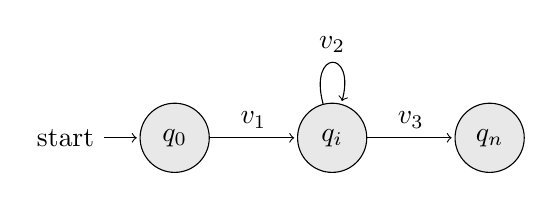
\begin{tikzpicture}[shorten >=1pt,node distance=2cm,on grid,auto]
      \tikzstyle{every state}=[fill={rgb:black,1;white,10}]
    
      \node[state,initial](q_0){$q_0$};
      \node[state](q_i)[right of=q_0]{$q_i$};
      \node[state](q_n)[right of=q_i]{$q_n$};    
      \path[->]
      (q_0) edge                node {$v_1$}  (q_i)
      (q_i) edge                node {$v_3$}  (q_n)
            edge  [loop above]  node {$v_2$}  ();
    \end{tikzpicture}\end{center}

Thus, we state \textbf{The Pumping Lemma} and provide a proof:

\begin{theorem}[The Pumping Lemma]
      Let $L$ be any regular language. Then there exists a $p>0$ (called the \textbf{pumping length} such that, for any string $s\in A^*$ such that $|s|>=p$, we can write \[s=s_1s_2s_3\] where 
      \begin{itemize}
            \item $|s_2|\geq 1$
            \item $|s_1s_2|\leq p$
            \item $L$ accepts $s_1s_2^ns_3$ for all $n\geq0$.
      \end{itemize}
\end{theorem}

\begin{proof}

\end{proof}

\subsubsection{Regular Grammars}
\begin{definition}
      A \textbf{Context-Free Grammar} is a quartuple $G=(N, T, P, S)$ where 
            \begin{align*}
                  & N\text{ is a finite, non-empty set of variables (also called non-terminals)}\\
                  & T\text{ is an alphabet of terminals}\\
                  & P\subseteq N\times(N\cup T)^*\text{ is a finite set of productions}\\
                  & S\in N\text{ is the starting symbol}
            \end{align*}

            For any $(A, \gamma)\in P$, we write $A\to\gamma$, and say $A$ \textbf{produces} $\gamma$. 
\end{definition}

By convention, we use upper-case letters to denote variables, lower-case to denote terminals and strings over the terminals, and Greek letters to denote strings over variables and terminals.

\begin{definition}
      Given strings $\alpha$ and $\beta$, we say $\alpha$ \textbf{derives} $\beta$ if there exist $A, \alpha_1,\alpha_2,\gamma$ such that 
      \begin{align*}
            \alpha &= \alpha_1A\alpha_2\\
            \beta  &= \alpha_1\gamma\alpha_2\\
            A&\to \gamma\in P
      \end{align*}

      and we write this $\alpha\Rightarrow\beta$. 
\end{definition}
\subsection{Accepted by Turing Machines}\label{subsec:accepted-by-turing-machine}
\subsection{Exercise Set 1}\label{subsec:exercise-set-1}

\begin{exercise}{1}
Construct DFAs for the following NFAs using the subset construction:
\begin{enumerate}[(a)]
\begin{multicols}{3}
    \item\begin{tabular}[t]{r|c r}
         & $a$ & \\\hline
    $\to 1$ & 2 & 0 \\
    2 & 3 & 0 \\
    3 & 4 & 0\\
    4 & 5 & 0\\
    5 & 6 & 0\\
    6 & 7 & 0\\
    7 & 1, 2 & 1
        \end{tabular}
    \item\begin{tabular}[t]{r| c c c r}
            & $a$ & $b$ & $c$ & \\\hline
        $\to 1$ & 2 & 2 & 2 & 1\\
              2 & 3 & 1 & 1, 2 & 1\\
              3 & 4 & 3 & $\emptyset$ & 1 \\
              4 & 5 & 4 & 4 & 1\\
              5 & 1 & 5 & 5 & 1
    \end{tabular}
    \item \begin{tabular}[t]{r| c c c r}
            & $a$ & $b$ & $c$ & \\\hline
        $\to 1$ & 2 & 2 & 2 & 1\\
              2 & 3 & 1 & 2, 3 & 1\\
              3 & 4 & 3 & $\emptyset$ & 1 \\
              4 & 5 & 4 & 4 & 1\\
              5 & 1 & 5 & 5 & 1
    \end{tabular}
\end{multicols}
\end{enumerate}
\end{exercise}

\begin{solution}\mbox{\\}
\begin{enumerate}[(a)]
\begin{multicols}{2}
    \item\begin{tabular}[t]{r|c r}
         & $a$ & \\\hline
            $\to1$ & 2 & 0 \\
            2 & 3 & 0 \\
            3 & 4 & 0\\
            4 & 5 & 0\\
            5 & 6 & 0\\
            6 & 7 & 0\\
            7 & 1, 2 & 1\\
            1, 2 & 2, 3 & 0\\
            2, 3 & 3, 4 & 0\\
            3, 4 & 4, 5 & 0\\
            4, 5 & 5, 6 & 0\\
            5, 6 & 6, 7 & 0\\
            6, 7 & 1, 2, 7 & 1\\
            1, 2, 7 & 1, 2, 3 & 1\\
            1, 2, 3 & 2, 3, 4 & 0\\
            2, 3, 4 & 3, 4, 5 & 0\\
            3, 4, 5 & 4, 5, 6 & 0\\
            4, 5, 6 & 5, 6, 7 & 0\\
            5, 6, 7 & 1, 2, 6, 7 & 1\\
            1, 2, 6, 7 & 1, 2, 3, 7 & 1\\
            1, 2, 3, 7 & 1, 2, 3, 4 & 1\\
            1, 2, 3, 4 & 2, 3, 4, 5 & 0\\
            2, 3, 4, 5 & 3, 4, 5, 6 & 0\\
            3, 4, 5, 6 & 4, 5, 6, 7 & 0\\
            4, 5, 6, 7 & 1, 2, 5, 6, 7 & 1\\
            1, 2, 5, 6, 7 & 1, 2, 3, 6, 7 & 1\\
            1, 2, 3, 6, 7 & 1, 2, 3, 4, 7 & 1\\
            1, 2, 3, 4, 7 & 1, 2, 3, 4, 5 & 1\\
            1, 2, 3, 4, 5 & 2, 3, 4, 5, 6 & 0\\
            2, 3, 4, 5, 6 & 3, 4, 5, 6, 7 & 0\\
            3, 4, 5, 6, 7 & 1, 2, 4, 5, 6, 7 & 1\\
            1, 2, 4, 5, 6, 7 & 1, 2, 3, 5, 6, 7 & 1\\
            1, 2, 3, 5, 6, 7 & 1, 2, 3, 4, 6, 7 & 1\\
            1, 2, 3, 4, 6, 7 & 1, 2, 3, 4, 5, 7 & 1\\
            1, 2, 3, 4, 5, 7 & 1, 2, 3, 4, 5, 6 & 1\\
            1, 2, 3, 4, 5, 6 & 2, 3, 4, 5, 6, 7 & 0\\
            2, 3, 4, 5, 6, 7 & 1, 2, 3, 4, 5, 6 7 & 1\\
            1, 2, 3, 4, 5, 6, 7 & 1, 2, 3, 4, 5, 6, 7 & 1
        \end{tabular}
        
        \item\begin{tabular}[t]{r|c c c r}
            & $a$ & $b$ & $c$ &\\\hline
               $\to1$ & 2 & 2 & 2 & 1\\
                2 & 3 & 1 & 1, 2 & 1\\
                3 & 4 & 3 & $\emptyset$ & 1\\
                1, 2 & 2, 3 & 1, 2 & 1, 2 & 1\\
                4 & 5 & 4 & 4 & 1\\
                $\emptyset$ & $\emptyset$ & $\emptyset$ & $\emptyset$ & 0\\
                2, 3 & 3, 4 & 1, 3 & 1, 2 & 1\\
                5 & 1 & 5 & 5 & 1\\
                3, 4 & 4, 5 & 3, 4 & 4 & 1\\
                1, 3 & 2, 4 & 2, 3 & 2 & 1\\
                4, 5 & 1, 5 & 4, 5 & 4, 5 & 1\\
                2, 4 & 3, 5 & 1, 4 & 1, 2, 4 & 1\\
                1, 5 & 1, 2 & 2, 5 & 2, 5 & 1\\
                3, 5 & 1, 4 & 3, 5 & 5 & 1\\
                1, 4 & 2, 5 & 2, 4 & 2, 4 & 1\\
                1, 2, 4 & 2, 3, 5 & 1, 2, 4 & 1, 2, 4 & 1\\
                2, 5 & 1, 3 & 1, 5 & 1, 2, 5 & 1\\
                2, 3, 5 & 1, 3, 4 & 1, 3, 5 & 1, 2, 5 & 1\\
                1, 2, 5 & 1, 2, 3 & 1, 2, 5 & 1, 2, 5 & 1\\
                1, 3, 4 & 2, 4, 5 & 2, 3, 4 & 2, 4 & 1\\
                1, 3, 5 & 1, 2, 4 & 2, 3, 5 & 2, 5 & 1\\
                1, 2, 3 & 2, 3, 4 & 1, 2, 3 & 1, 2 & 1\\
                2, 4, 5 & 1, 3, 5 & 1, 4, 5 & 1, 2, 4, 5 & 1\\
                2, 3, 4 & 3, 4, 5 & 1, 3, 4 & 1, 2, 4 & 1\\
                1, 4, 5 & 1, 2, 5 & 2, 4, 5 & 2, 4, 5 & 1\\
                1, 2, 4, 5 & 1, 2, 3, 5 & 1, 2, 4, 5 & 1, 2, 4, 5 & 1\\
                3, 4, 5 & 1, 4, 5 & 3, 4, 5 & 4, 5 & 1\\
                1, 2, 3, 5 & 1, 2, 3, 4 & 1, 2, 3, 5 & 1, 2, 5 & 1\\
                1, 2, 3, 4 & 2, 3, 4, 5 & 1, 2, 3, 4 & 1, 2, 4 & 1\\
                2, 3, 4, 5 & 1, 3, 4, 5 & 1, 3, 4, 5 & 1, 2, 4, 5 & 1\\
                1, 3, 4, 5 & 1, 2, 4, 5 & 2, 3, 4, 5 & 2, 4, 5 & 1
           \end{tabular}
\end{multicols}

\item\begin{tabular}[t]{r|c c c r}
    & $a$ & $b$ & $c$ &\\\hline
       $\to1$ & 2 & 2 & 2 & 1\\
       2 & 3 & 1 & 2, 3 & 1\\
       3 & 4 & 3 & $\emptyset$ & 1\\
       2, 3 & 3, 4 & 1, 3 & 2, 3 & 1\\
       4 & 5 & 4 & 4 & 1\\
       $\emptyset$ & $\emptyset$ & $\emptyset$ & $\emptyset$ & 0\\
       3, 4 & 4, 5 & 3, 4 & 4 & 1\\
       1, 3 & 2, 4 & 2, 3 & 2 & 1\\
       5 & 1 & 5 & 5 & 1\\
       4, 5 & 1, 5 & 4, 5 & 4, 5 & 1\\
       2, 4 & 3, 5 & 1, 4 & 2, 3 & 1\\
       1, 5 &6& 2, 5 & 2, 5 & 1\\
       3, 5 & 1, 4 & 3, 5 & 5 & 1\\
       1, 4 & 2, 5 & 2, 4 & 2, 4 & 1\\
       6 & 2, 3 & 1, 2 & 2, 3 & 1\\
       2, 5 & 1, 3 & 1, 5 & 2, 3, 5 & 1\\
       2, 3, 5 & 1, 3, 4 & 1, 3, 5 & 2, 3, 5 & 1\\
       1, 3, 4 & 2, 4, 5 & 2, 3, 4 & 2, 4 & 1\\
       1, 4, 5 & 1, 2, 4 & 2, 4, 5 & 2, 4, 5 & 1\\
       2, 4, 5 & 1, 3, 5 & 1, 4, 5 & 2, 3, 4, 5 & 1\\
       2, 3, 4 & 3, 4, 5 & 1, 3, 4 & 2, 3, 4 & 1\\
       1, 2, 4 & 2, 3, 5 & 1, 2, 4 & 2, 3, 4 & 1\\
       1, 3, 5 & 1, 2, 4 & 2, 3, 5 & 2, 5 & 1\\
       2, 3, 4, 5 & 1, 3, 4, 5 & 1, 3, 4, 5 & 2, 3, 4, 5 & 1\\
       3, 4, 5 & 1, 4, 5 & 3, 4, 5 & 4, 5 & 1\\
       1, 3, 4, 5 & 1, 2, 4, 5 & 2, 3, 4, 5 & 2, 4, 5 & 1\\
       1, 2, 4, 5 & 1, 2, 3, 5 & 1, 2, 4, 5 & 2, 3, 4, 5 & 1\\
       1, 2, 3, 5 & 1, 2, 3, 4 & 1, 2, 3, 5 & 2, 3, 5 & 1\\
       1, 2, 3, 4 & 2, 3, 4, 5 & 1, 2, 3, 4 & 2, 3, 4 & 1\\
   \end{tabular}
\end{enumerate}
\end{solution}

\begin{exercise}{2}
Reduce the following DFAs:
\begin{enumerate}[(a)]
\begin{multicols}{3}
    \item \begin{tabular}[t]{c c| c c r}
         & & $a$ & $b$ & \\\hline
         $\to$ & 1 & 2 & 3 & 0\\
               & 2 & 3 & 2 & 1\\
               & 3 & 4 & 5 & 0\\
               & 4 & 1 & 8 & 1\\
               & 5 & 6 & 7 & 0\\
               & 6 & 7 & 6 & 1\\
               & 7 & 8 & 1 & 0\\
               & 8 & 5 & 4 & 1
    \end{tabular}
    
    \item \begin{tabular}[t]{c c| c c r}
         & & $a$ & $b$ & \\\hline
         $\to$ & 1 & 2 & 3 & 0\\
               & 2 & 3 & 2 & 1\\
               & 3 & 4 & 5 & 0\\
               & 4 & 1 & 8 & 1\\
               & 5 & 6 & 7 & 0\\
               & 6 & 7 & 6 & 1\\
               & 7 & 8 & 1 & 0\\
               & 8 & 5 & 5 & 1
    \end{tabular}
    
    \item Your result of 1(b).
    
    \item Your result of 1(c).
\end{multicols}
\end{enumerate}
\end{exercise}

\begin{solution}\mbox{\\}
    \begin{enumerate}[(a)]
        \begin{multicols}{2}
            \item \begin{tabular}[t]{|c|c|c|c|c|c|c|c|}\hline
                \multicolumn{4}{|c|}{Rejecting} & \multicolumn{4}{|c|}{Accepting}\\\hline
                \multicolumn{4}{|c|}{1, 3, 5, 7} & \multicolumn{4}{|c|}{2, 4, 6, 8}\\\hline
                \multicolumn{4}{|c|}{1, 3, 5, 7} & \multicolumn{4}{|c|}{2, 4, 6, 8}\\\hline
                \end{tabular}

                Setting $p=\{1, 3, 5, 7\}$ and $q=\{2, 4, 6, 8\}$:

                \begin{tabular}{r| c c r}
                    & $a$ & $b$ & \\\hline
                    $\to p$ & $q$ & $p$ & 0\\
                          $q$ & $p$ & $q$ & 1\\
               \end{tabular}
               
            \item \begin{tabular}[t]{|c|c|c|c|c|c|c|c|}\hline
                \multicolumn{4}{|c|}{Rejecting} & \multicolumn{4}{|c|}{Accepting}\\\hline
                \multicolumn{4}{|c|}{1, 3, 5, 7} & \multicolumn{4}{|c|}{2, 4, 6, 8}\\\hline
                \multicolumn{4}{|c|}{1, 3, 5, 7} & \multicolumn{3}{|c|}{2, 4, 6} & \multicolumn{1}{c|}{8}\\\hline
                \multicolumn{3}{|c}{1, 3, 5} & \multicolumn{1}{|c|}{7} & \multicolumn{2}{|c}{2, 6} & \multicolumn{1}{|c|}{4} & \multicolumn{1}{c|}{8}\\\hline
                1 & 3 & 5 & \multicolumn{1}{c|}{7} & \multicolumn{1}{|c|}{2} & 6 & 4 & 8\\\hline
                \end{tabular}
                
                The DFA is already reduced.
        \end{multicols}
    \item We will rename the states for simplicity:

        \begin{center}\begin{tabular}{r|c c c r}
            & $a$ & $b$ & $c$ &\\\hline
               $\to1$ & 2 & 2 & 2 & 1\\
                2 & 3 & 1 & 6 & 1\\
                3 & 4 & 3 & 0 & 1\\
                6 & 7 & 6 & 6 & 1\\
                4 & 5 & 4 & 4 & 1\\
                0 & 0 & 0 & 0 & 0\\
                7 & 8 & 9 & 6 & 1\\
                5 & 1 & 5 & 5 & 1\\
                8 & 10 & 8 & 4 & 1\\
                9 & 1 & 7 & 2 & 1\\
                10 & 12 & 10 & 10 & 1\\
                11 & 13 & 14 & 15 & 1\\
                12 & 6 & 16 & 16 & 1\\
                13 & 14 & 13 & 5 & 1\\
                14 & 16 & 11 & 11 & 1\\
                15 & 17 & 15 & 15 & 1\\
                16 & 9 & 12 & 18 & 1\\
                17 & 19 & 20 & 18 & 1\\
                18 & 21 & 18 & 18 & 1\\
                19 & 22 & 23 & 11 & 1\\
                20 & 15 & 17 & 16 & 1\\
                21 & 23 & 21 & 6 & 1\\
                22 & 20 & 24 & 25 & 1\\
                23 & 26 & 19 & 15 & 1\\
                24 & 18 & 22 & 22 & 1\\
                25 & 27 & 25 & 25 & 1\\
                26 & 24 & 26 & 10 & 1\\
                27 & 28 & 27 & 18 & 1\\
                28 & 29 & 28 & 15 & 1\\
                29 & 30 & 30 & 25 & 1\\
                30 & 25 & 29 & 22 & 1
           \end{tabular}\end{center}

           \begin{center}\begin{tabular}[t]{|c|c|c|c|c|c|c|c|c|c|c|c|c|c|c|c|c|c|c|c|c|c|c|c|c|c|c|c|c|c|c|}\hline
            \multicolumn{1}{|c|}{Rejecting} & \multicolumn{30}{|c|}{Accepting}\\\hline
            \multicolumn{1}{|c|}{0} & \multicolumn{30}{|c|}{$1,2,3,\hdots,30$}\\\hline
            \multicolumn{1}{|c|}{0} & \multicolumn{29}{|c|}{$1,2,4,5,\hdots,30$} & 3\\\hline
            \multicolumn{1}{|c|}{0} & \multicolumn{28}{|c|}{$1,4,5,\hdots,30$} & 2 & 3\\\hline
            \multicolumn{1}{|c|}{0} & \multicolumn{26}{|c|}{$4,5,6,7,8,10,\hdots,30$} & \multicolumn{1}{c|}{1} & \multicolumn{1}{c|}{9} & 2 & 3\\\hline
            \multicolumn{1}{|c|}{0} & \multicolumn{22}{|c|}{$4,6,8,10,\hdots,30$} & \multicolumn{1}{c|}{13} & \multicolumn{1}{c|}{16} & \multicolumn{1}{c|}{7} & \multicolumn{1}{c|}{5} & \multicolumn{1}{c|}{1} & \multicolumn{1}{c|}{9} & 2 & 3\\\hline
            \end{tabular}\end{center}
    \end{enumerate}
\end{solution}

\begin{exercise}{3}
Construct NFAs for the following regular expressions using the construction given in class; then find the corresponding DFAs; then reduce them:
\begin{enumerate}[(a)]
\begin{multicols}{2}
    \item $(a^2 \cup a^3 \cup a^5)^*$ over $\{a\}$
    \item $(a^2)^*(a^3)^*(a^5)^*$ over $\{a\}$
    \item $(abc \cup ab)^*aa^*(ab)^*$ over $\{a, b, c\}$
    \item $0^*(00\cup11)^*(01\cup10)^*1^*$ over $\{0, 1\}$
\end{multicols}
\end{enumerate}
\end{exercise}

\begin{exercise}{4}
Construct regular expressions for the languages accepted by the following automata:
\begin{enumerate}[(a)]
\begin{multicols}{2}
    \item \begin{tabular}[t]{c c| c c c c}
         & & $a$ & $b$ & $c$ & \\\hline
         $\to$ & 1 & 2 & 2 & 2 & 1\\
               & 2 & 3 & 1 & 2, 3 & 1\\
               & 3 & 4 & 3 & $\emptyset$ & 1\\
               & 4 & 1 & 4 & 4 & 1
    \end{tabular}
    \item \begin{tabular}[t]{c c| c c c}
         & & $a$ & $b$ & \\\hline
         $\to$ & $A$ & $B$ & $C$ & 0\\
               & $B$ & $A$ & $C$ & 0\\
               & $C$ & $B$ & $A$ & 1 
    \end{tabular}
\end{multicols}
\end{enumerate}
\end{exercise}

\begin{solution}
    \begin{enumerate}[(a)]
        \item 
        
        \begin{align*}
            X_1 &= aX_2\cup bX_2\cup cX_2\cup\varepsilon\\
            X_2 &= aX_3\cup bX_1 \cup c(X_2\cup X_3)\cup\varepsilon\\
            X_3 &= aX_4\cup bX_3\cup\varepsilon\\
            X_4 &= aX_1\cup bX_4\cup cX_4\cup\varepsilon  
        \end{align*}
        Solving for $X_4$ 
        \begin{align*}
            X_4 &= aX_1\cup bX_4\cup cX_4\cup\varepsilon\\
                &= aX_1\cup (b\cup c)X_4\cup\varepsilon\\
                &= (b\cup c)X_4\cup aX_1\cup\varepsilon\\
                &= (b\cup c)^*\cup aX_1\cup\varepsilon\\
                &= (b\cup c)^*(\varepsilon\cup aX_1)\\
                &= (b\cup c)^*\cup (b\cup c)^*aX_1
        \end{align*}
    Similarly, 
        \begin{align*}
            X_3 &= aX_4\cup bX_3\cup\varepsilon\\
                &= a\left((b\cup c)^*\cup (b\cup c)^*aX_1\right)\cup bX_3\cup\varepsilon\\
                &= bX_3\cup a\left((b\cup c)^*\cup (b\cup c)^*aX_1\right)\cup\varepsilon\\
                &= b^*(a\left((b\cup c)^*\cup (b\cup c)^*aX_1\right)\cup\varepsilon)\\
                &= b^*a(b\cup c)^*\cup b^*(b\cup c)^*aX_1\cup b^*
        \end{align*}
    Solving $X_2$:
    \begin{align*}
        X_2 &= aX_3\cup bX_1 \cup c(X_2\cup X_3)\cup\varepsilon\\
            &= (a\cup c)X_3 \cup bX_1 \cup cX_2\cup\varepsilon
    \end{align*}

    Finally, solving for $X_1$:
    \begin{align*}
        X_1 &= aX_2\cup bX_2\cup cX_2\cup\varepsilon\\
            &= (a\cup b\cup c)X_2\cup\varepsilon\\
            &= (a\cup b\cup c)c^*\cup (a\cup c)(b^*\cup a(b\cup c)^*\cup a\cup\varepsilon)\cup\varepsilon\cup((a\cup c)a^2\cup b)X_1\cup\varepsilon\\
            &= ((a\cup c)a^2\cup b)^*\cup(a\cup b\cup c)c^*\cup (a\cup c)(b^*\cup a(b\cup c)^*\cup a\cup\varepsilon)
    \end{align*}
        \item
    \begin{align*}
        X_A &= aX_B\cup bX_C\\
        X_B &= aX_A\cup bX_C\\
        X_C &= aX_B\cup bX_A\cup\varepsilon
    \end{align*}
    Plugging in the equation for $X_C$ into $X_B$
    \begin{align*}
        X_B &= aX_A\cup b(aX_B\cup bX_A\cup\varepsilon)\\
            &= aX_A\cup baX_B\cup b^2X_A\cup b\\
            &= baX_b\cup aX_A\cup b^2X_A\cup b\\
            &= (ba)^*\cup aX_A\cup b^2X_A\cup b\\
            &= (ba)^*\cup b\cup (a\cup b^2)X_A
    \end{align*}
    We substitute back into $X_C$:
    \begin{align*}
        X_C &= a((ba)^*\cup b\cup (a\cup b^2)X_A)\cup bX_A\cup\varepsilon\\
            &= a(ba)^*\cup ab\cup (a^2\cup ab^2)X_A\cup bX_A\cup\varepsilon\\
            &= a(ba)^*\cup ab\cup (a^2\cup ab^2\cup b)X_A\cup\varepsilon
    \end{align*}
    We now substitute the new equations for $X_B$ and $X_C$ into the equation for $X_A$
    \begin{align*}
        X_A &= a\left((ba)^*\cup b\cup (a\cup b^2)X_A\right)\cup b(a(ba)^*\cup ab\cup (a^2\cup ab^2\cup b)X_A\cup\varepsilon)\\
            &= a(ba)^*\cup ab\cup a^2\cup ab^2X_A\cup ba(ba)^*\cup bab \cup (ba^2\cup bab^2\cup b^2)X_A\cup b\\
            &= (ab^2\cup ba^2\cup bab^2\cup b^2)X_A\cup a(ba)^*\cup ab\cup a^2\cup ba(ba)^*\cup bab \cup b\\
            &= (ab^2\cup ba^2\cup bab^2\cup b^2)^*\cup a(ba)^*\cup ab\cup a^2\cup ba(ba)^*\cup bab \cup b
    \end{align*}
    \end{enumerate}
\end{solution}

\subsection{Exercise Set 2}\label{subsec:exercise-set-2}
\begin{exercise}{1}
    Prove that the following languages are not regular:
    \begin{enumerate}[(a)]
        \item \(L=\{x\in{(0\cup1)}^*2{(0\cup1)}^*|\text{number of 0s before 2} = \text{number of 1s after 2}\} \)
        \item \(L=\{x\in{(0\cup1)}^*2{(0\cup1)}^*|\text{number of 0s before 2} \neq \text{number of 1s after 2}\} \)
        \item \(L=\{a^{i^2}|i\geq1\} \)
        \item \(L=\{a^{2^i}|i\geq1\} \)
    \end{enumerate}
\end{exercise}
\begin{solution}\mbox{\\}
\begin{enumerate}[(a)]
    \item Suppose, by way of contradiction, that \(L\) is regular and that \(p\) is its pumping length. Consider the string \(s=0^p21^p\). Clearly, \(|s|\geq p\). Thus, by the \textbf{Pumping Lemma}, there exist strings \(s_1, s_2, s_3\) such that \(s=s_1s_2s_3\) with \(|s_1s_2|\leq p\) and \(|s_2|\geq1\) and, for all \(n\geq 0\), \(s_1s_2^n s_3\in L\). Observe that \(s_1s_2=0^k\) for some \(k\leq p\) (for otherwise \(|s_1s_2| > p\)), hence \(s_3=0^{p-k}21^p\). Thus, we write \(s_1=0^{k-q}\) and \(s_2=0^{q}\) for some \(q\geq1\). By the pumping lemma, 
    \begin{align*}
        s_1s_2^n s_3 &= 0^{k-q}{(0^q)}^n0^{p-k}21^p\\
                    &= 0^{k-q}0^{qn}0^{p-k}21^p\\
                    &= 0^{p+q(n-1)}21^p
    \end{align*}

    is in \(L\). However, for \(n\geq2\), there are more 0s before the 2 than 1s after, hence \(s_1s_2^n s_3\not\in L\). A contradiction. Thus, \(L\) is not regular.

    \item Suppose, by way of contradiction, that \(L\) is regular and that \(p\) is its pumping length. Consider the string \(s=0^p21^{p+p!}\). Clearly, \(|s|\geq p\). Thus, by the \textbf{Pumping Lemma}, there exist strings \(s_1\), \(s_2\), \(s_3\) such that \(s=s_1s_2s_3\) with \(|s_1s_2|\leq p\) and \(|s_2|\geq1\) and, for all \(n\geq 0\), \(s_1s_2^n s_3\in L\). Observe that \(s_1s_2=0^k\) for some \(k\leq p\) (for otherwise \(|s_1s_2| > p\)), hence \(s_3=0^{p-k}21^{p+p!}\). Thus, we write \(s_1=0^{k-q}\) and \(s_2=0^{q}\) for some \(q\geq1\). By the pumping lemma, 
    \begin{align*}
        s_1s_2^n s_3 &= 0^{k-q}{(0^q)}^n0^{p-k}21^{p+p!}\\
                    &= 0^{k-q}0^{qn}0^{p-k}21^{p+p!}\\
                    &= 0^{p+q(n-1)}21^{p+p!}
    \end{align*}

    is in \(L\). Now, since \(q\leq p\), \(q\mid p{!}\). Thus, taking \(n=\frac{p!}{q}+1\), we have 
    \begin{align*}
        s_1s_2^n s_3 &= 0^{p+q(\frac{p!}{q}+1-1)}21^{p+p!}\\
                    &= 0^{p+q(\frac{p!}{q})}21^{p+p!}\\
                    &= 0^{p+p!}21^{p+p!}
    \end{align*}
    
    Thus, \(s_1s_2^n s_3\not\in L\), a contradiction. Therefore \(L\) is not regular.
    \item In order to reach a contradiction, suppose \(L\) is regular and that \(p\) is its pumping length. Consider the string \(s=a^{p^2}\). By the pumping lemma, we have \(s=s_1s_2s_3\). Since \(|s_1s_2|\leq p\), this forces \(s_1s_2=a^k\) for some \(0<k\leq p\) and \(s_3=a^{p^2-k}\). Then \(s_1=a^{k-r}\) and \(s_2=a^r\) for some \(0<r\leq k\). Then
    \begin{align*}
        s_1s_2^n s_3 &= a^{k-r}{(a^r)}^n a^{p^2-k}\\
                    &= a^{k-r}a^{rn}a^{p^2-k}\\
                    &= a^{p^2+rn-r}\\
                    &= a^{p^2+r(n-1)}
    \end{align*}
    Take \(n=2\). Then \(s_1s_2^n s_3=a^{p^2+r}\in L\). However, \(p^2+r\) cannot be a perfect square: since \(r \leq p\), we have 
    \begin{align*}
        p^2+r &\leq p^2 + p\\
              &< p^2 + p + 1\\
              &= {(p+1)}^2
    \end{align*}
    
    Thus, \(s_1s_2^n s_3\not\in L\), a contradiction. Therefore \(L\) is not regular.
    \item In order to reach a contradiction, suppose \(L\) is regular and that \(p\) is its pumping length. Consider the string \(s=a^{2^p}\). By the pumping lemma, we have \(s=s_1s_2s_3\). Since \(|s_1s_2|\leq p\), this forces \(s_1s_2=a^k\) for some \(0<k\leq p\) and \(s_3=a^{2^p-k}\). Then \(s_1=a^{k-r}\) and \(s_2=a^r\) for some \(0<r\leq k\). Then
    \begin{align*}
        s_1s_2^n s_3 &= a^{k-r}{(a^r)}^n a^{2^p-k}\\
                    &= a^{k-r}a^{rn}a^{2^p-k}\\
                    &= a^{2^p+rn-r}\\
                    &= a^{2^p+r(n-1)}
    \end{align*}
    Take \(n=2\). Then \(s_1s_2^n s_3=a^{2^p+r}\in L\). However, \(2^p+r\) cannot be a power of 2: since \(r \leq p\), we have 
    \begin{align*}
        2^p+r &\leq 2^p + p\\
              &< 2^p + 2^p\\
              &= 2^{p+1}
    \end{align*}
    
    Thus, \(s_1s_2^n s_3\not\in L\), a contradiction. Therefore \(L\) is not regular.
\end{enumerate}
    
\end{solution}

\begin{exercise}{2}
    Construct DFAs for the following extended regular expressions:
    \begin{enumerate}[(a)]
        \item \(\left[\overline{{(000)}^*}\cap\left({(01)}^*\cup{(10)}^*\right)\right]\cap\overline{{(11)}^*}\) over \( \{0,1\} \)
        \item \(\overline{{(0\cup1)}^*01^*10^*01^*1{(0\cup1)}^*} - {(10\cup01)}^*\) over \( \{0, 1, 2\} \)
    \end{enumerate}
\end{exercise}

\begin{exercise}{3}
    Construct Chomsky Normal Form grammars for \(L(G)-\varepsilon \) for the following cfgs \(G\):
    \begin{enumerate}[(a)]
        \item \(G=\left(\{a, b\}, \{S, A\}, S, \{S\to aAAaS\mid a, A\to bAA\mid aSSSA\mid \varepsilon \}\right)\)
        \item \(G=\left(\{a, b, c\}, \{S, A, B\}, S, \{S\to aAA\mid A, A\to bBBB\mid B\mid \varepsilon, B\to bSSS\mid S\mid \varepsilon \}\right)\)
    \end{enumerate}
\end{exercise}

\begin{solution}\mbox{\\}
    \begin{enumerate}[(a)]
        \item 
        \begin{align*}
            S &\to aAAaS\mid a\\
            A &\to bAA\mid aSSSA\mid \varepsilon 
        \end{align*}

        There are no useless productions, since \(S\Rightarrow a\) and \(A\Rightarrow b\). \(A\) is clearly nullable, so we get  

        \begin{align*}
            S &\to aAAaS\mid a{\color{red}\cancel{A}}AaS\mid aA{\color{red}\cancel{A}}aS\mid a{\color{red}\cancel{A}}{\color{red}\cancel{A}}aS\mid a\\
            A &\to bAA\mid b{\color{red}\cancel{A}}A\mid bA{\color{red}\cancel{A}}\mid b{\color{red}\cancel{A}}{\color{red}\cancel{A}} \mid aSSSA\mid aSSS{\color{red}\cancel{A}} 
        \end{align*}

        which reduces to 

        \begin{align*}
            S &\to aAAaS\mid aAaS\mid aaS\mid a\\
            A &\to bAA\mid bA\mid b \mid aSSSA\mid aSSS 
        \end{align*}
        There are no unit productions. Setting \(X_a\to a\) and \(X_b\to b\), we have 

        \begin{align*}
            S &\to X_a AAX_a S\mid X_a AX_a S\mid X_a X_a S\mid a\\
            A &\to X_b AA\mid X_b A\mid b \mid X_a SSSA\mid X_a SSS 
        \end{align*}

        Finally, we decompose:

        \begin{align*}
            S &\to X_a S_1\mid X_a S_2\mid X_a S_3\mid a\\
            A &\to X_b A_1\mid X_b A\mid b \mid X_a A_2\mid X_a A_5 \\
            S_1 &\to AS_2\\
            S_2 &\to AS_3\\
            S_3 &\to X_a S\\
            A_1 &\to AA\\
            A_2 &\to SA_3\\
            A_3 &\to SA_4\\
            A_4 &\to SA\\
            A_5 &\to SA_6\\
            A_6 &\to SS
        \end{align*}

        \item 
        \begin{align*}
            S &\to aAA\mid A\\ 
            A &\to bBBB\mid B\mid \varepsilon \\
            B &\to bSSS\mid S\mid \varepsilon 
        \end{align*}

        There are no useless productions, since \(S\Rightarrow a\), \(A\Rightarrow b\) and \(B\Rightarrow b\). Clearly, \(S\), \(A\), and \(B\) are all nullable. Thus, we have 

        \begin{align*}
            S &\to aAA\mid a{\color{red}\cancel{A}}\mid aA{\color{red}\cancel{A}}\mid a{\color{red}\cancel{A}}{\color{red}\cancel{A}}\mid A\mid {\color{red}\cancel{A}}\\ 
            A &\to bBBB\mid b{\color{red}\cancel{B}}BB\mid bB{\color{red}\cancel{B}}B\mid bBB{\color{red}\cancel{B}}\mid b{\color{red}\cancel{B}}{\color{red}\cancel{B}}B\mid b{\color{red}\cancel{B}}B{\color{red}\cancel{B}}\mid bB{\color{red}\cancel{B}}{\color{red}\cancel{B}}\mid B\mid {\color{red}\cancel{B}}\\
            B &\to bSSS\mid b{\color{red}\cancel{S}}SS\mid bS{\color{red}\cancel{S}}S\mid bSS{\color{red}\cancel{S}}\mid b{\color{red}\cancel{S}}{\color{red}\cancel{S}}S\mid b{\color{red}\cancel{S}}S{\color{red}\cancel{S}}\mid bS{\color{red}\cancel{S}}{\color{red}\cancel{S}}\mid b{\color{red}\cancel{S}}{\color{red}\cancel{S}}{\color{red}\cancel{S}}\mid S\mid {\color{red}\cancel{S}} 
        \end{align*}

        which reduces to

        \begin{align*}
            S &\to aAA\mid a\mid aA\mid A \\ 
            A &\to bBBB\mid bBB\mid bB\mid B \\
            B &\to bSSS\mid bSS\mid bS\mid b\mid S  
        \end{align*}

        We eliminate the unit productions \(S\to A\), \(A\to B\) and \(B\to S\).

        \begin{align*}
            S &\to aAA\mid a\mid aA\mid bBBB\mid bBB\mid bB \\ 
            A &\to bBBB\mid bBB\mid bB\mid bSSS\mid bSS\mid bS\mid b \\
            B &\to bSSS\mid bSS\mid bS\mid b\mid aAA\mid a\mid aA\mid bBBB\mid bBB\mid bB
        \end{align*}

        We now set \(X_a\to a\) and \(X_b\to b\):

        \begin{align*}
            S &\to X_a AA\mid a\mid X_a A\mid X_b BBB\mid X_b BB\mid X_b B \\ 
            A &\to X_b BBB\mid X_b BB\mid X_b B\mid X_b SSS\mid X_b SS\mid X_b S\mid b \\
            B &\to X_b SSS\mid X_b SS\mid X_b S\mid b\mid X_a AA\mid a\mid X_a A\mid X_b BBB\mid X_b BB\mid X_b B
        \end{align*}

        Finally, we decompose:

        \begin{align*}
            S &\to X_a S_1\mid a\mid X_a A\mid X_b S_2\mid X_b S_3\mid X_b B \\ 
            A &\to X_b S_2\mid X_b S_3\mid X_b B\mid X_b A_1\mid X_bA_2\mid X_b S\mid b \\
            B &\to X_b A_1\mid X_b A_2\mid X_b S\mid b\mid X_a S_1\mid a\mid X_a A\mid X_b S_2\mid X_b S_3\mid X_b B\\
            S_1 &\to AA\\
            S_2 &\to BS_3\\
            S_3 &\to BB\\
            A_1 &\to SA_2\\
            A_2 &\to SS\\
        \end{align*}
    \end{enumerate}
\end{solution}

\begin{exercise}{4}
    Construct Greibach Normal Form grammars for \(L(G)-\varepsilon \) for the following cfgs \(G\):
    \begin{enumerate}[(a)]
        \item \(G=\left(\{a, b\}, \{S, A, B\}, S, \{S\to SaS\mid A, A\to AAAb\mid B\mid \varepsilon, B\to SSS\mid a \}\right)\)
        \item \(G=\left(\{a, b\}, \{S, A, B, C\}, S, \{S\to ASS\mid a, A\to bBBB\mid BAA\mid \varepsilon, B\to CSS\mid SSC, C\to SS\mid b\}\right)\)
    \end{enumerate}
\end{exercise}

\begin{solution}\mbox{\\}
    \begin{enumerate}[(a)]
        \item 
        \begin{align*}
            S &\to SaS\mid A\\
            A &\to AAAb\mid B\mid \varepsilon \\
            B &\to SSS\mid a
        \end{align*}
        There are no useless productions, since \(B\Rightarrow a\), \(A\Rightarrow b\), and \(S\Rightarrow b\). We eliminate \(\varepsilon \) productions:
        
        \begin{align*}
            S &\to SaS\mid A\mid {\color{red}\cancel{A}}\\
            A &\to AAAb\mid {\color{red}\cancel{A}}AAb\mid A{\color{red}\cancel{A}}Ab\mid AA{\color{red}\cancel{A}}b\mid {\color{red}\cancel{A}}{\color{red}\cancel{A}}Ab\mid {\color{red}\cancel{A}}A{\color{red}\cancel{A}}b\mid A{\color{red}\cancel{A}}{\color{red}\cancel{A}}b\mid {\color{red}\cancel{A}}{\color{red}\cancel{A}}{\color{red}\cancel{A}}b\mid B \\
            B &\to SSS\mid a
        \end{align*}

        which reduces to

        \begin{align*}
            S &\to SaS\mid A\\
            A &\to AAAb\mid AAb\mid Ab\mid b\mid B \\
            B &\to SSS\mid a
        \end{align*}
        
        We now remove the unit productions, \(S\to A\) and \(A\to B\):

        \begin{align*}
            S &\to SaS\mid AAAb\mid AAb\mid Ab\mid b\\
            A &\to AAAb\mid AAb\mid Ab\mid b\mid SSS\mid a \\
            B &\to SSS\mid a
        \end{align*}
        
        \item 
        \begin{align*}
            S &\to ASS\mid a\\
            A &\to bBBB\mid BAA\mid \varepsilon \\
            B &\to CSS\mid SSC\\
            C &\to SS\mid b
        \end{align*}
    \end{enumerate}
\end{solution}
\section{Exam Cheatsheets}
\subsection{Exam 1}\label{subsec:exam-1-cheatsheet}
\subsubsection{Converting an NFA to a DFA}
Begin with the initial state. Apply the transitions and add any newly visited states. Stop when no new states can be visited. 

\subsubsection{Reducing a DFA}
Partition all states into accepting vs rejecting. Apply all transitions to a ``representative'' from a partition, then apply the transitions to the remaining members of the partition. If a member differs, move it to a new partition. 
\subsubsection{Converting a Regular Expression to an NFA}
\begin{enumerate}

\item[NFA for \(a\):]\begin{center}\begin{tabular}{r c c r}
    & \(a\) & \(b\neq a\) & \\\bottomrule
    \(\to q_0\) & \(q_1\) & \(\emptyset \) & 0\\
    \(q_1\) & \(\emptyset \) & \(\emptyset \) & 1\\
\end{tabular}\end{center}

\item[NFA for \(\varepsilon \):]\begin{center}\begin{tabular}{r c r}
    & \(c\in A\) & \\\bottomrule
    \(\to q_0\) & \(\emptyset \) & 1\\
\end{tabular}\end{center}

\item[NFA for \(\emptyset \):]\begin{center}\begin{tabular}{r c r}
    & \(c\in A\) & \\\bottomrule
    \(\to q_0\) & \(\emptyset \) & 0\\
\end{tabular}\end{center}
\end{enumerate}

\begin{center}\textbf{Union}\end{center} 

Union initial states, copy remaining states from \(\alpha \) and \(\beta \). Final states are final states from \(\alpha \) and \(\beta \). 

\begin{center}\textbf{Concatenation}\end{center}

For final states of \(\alpha \), union the state from \(\alpha \) with the initial state from \(\beta \). Copy non-final states from \(\alpha \) and non-initial states from \(\beta \). Final states:

If the initial state is rejecting in \(\beta \), final states are final states from \(\beta \). 

If the initial state is accepting in \(\beta \), final states are final states from \(\alpha \) and \(\beta \), except the initial state in \(\beta \). 

\begin{center}\textbf{Kleene Closure}\end{center}

Union final states with the initial state. Copy non-final states. Final states are final states from \(\alpha \) and the initial state.

\subsubsection{Converting an NFA to a Regular Expression}

Set up system of equations. Solve for equation corresponding to initial state. Remember the lemma: if \[X=LX\cup M\] then \[X=L^*M\]
\end{document}